
\section{重積分}
多変数関数の微分が偏微分ならば,多変数関数の積分は重積分である.
1変数関数の積分のところで,積分とは無限個の足し算であるという話をした.
これは,足していくものが1つの変数$x$だけで対応づけできるようなものであった.
ここから推察されるのは,重積分が複数の変数に対応づけされるようなものの無限個の足し算であるということである.
変数がいくつあっても議論はたいして変わらないので,とりあえず2変数でやってみよう.

\subsection{重積分の定義}
2変数関数$z=f(x, \, y)$を考えよう.まず,$x, \, y$の微小変化$\mathrm{d}x, \, \mathrm{d}y$を考え,
それらと$f(x, \, y)$の積$f(x, \, y) \: \mathrm{d}x\mathrm{d}y$を考える.そして,ある範囲$D$上でその総和をとる.
この和のことを
$$
\iint_{D} f(x, \, y) \: \mathrm{d}x\mathrm{d}y
$$
と書き表し,\emph{重積分}\index[widx]{じゅうせきぶん@重積分}と呼ぶのである.
変数が2つなので今は2重積分である.
$\int$記号が2つついているので$\iint$記号は``ダブル・インテグラル''とでも読んでおけばよい.
$\iiint$ならば``トリプル・インテグラル''である.

重積分が1変数関数の積分のときと非常によく似ているのがわかるだろうか? 違うのは
足していくものが$x$,$y$の2つの変数によって決定されるということである.

\subsubsection{``$D$上で総和をとる''とは?}
いまさっき説明したところで``ある範囲$D$上でその総和をとる''という言葉を使った.
これがどういう意味か分かるだろうか? 1変数関数においては$x$をいくつからいくつに変化させるかについてのみ考えればよかった.
しかし,2つ以上の変数についてはもう少し状況が複雑である.$x$の変化と$y$の変化を同時に考えなければならないからだ.
$x$と$y$がどう変化するかという情報を$D$という1文字で代表させているというわけだ.
変数は通常連続的に変化させるので$D$は2変数においてはある種の平面図形を形作る.
3変数においては空間図形である.そういうわけで,$D$は\emph{領域}と呼ばれる.
このように表記しておくと変数が増えたときに書き方を変えずに済む.
\subsection{2重積分は体積か}
1変数関数の積分のところで``積分とは面積を求める操作だと解釈できる''という話をした.
重積分においても同じようなことがいえるのである.
変数の数によって面積か体積かが変わるのでまずは2変数関数についてやろう.

$\mathrm{d}x, \, \mathrm{d}y$とはそれぞれ$x, \, y$の微分であった.今は``変化''という言葉から少し離れて
$\mathrm{d}x, \, \mathrm{d}y$を``微小の長さ''だと思ってみよう.
そうすると,$\mathrm{d}x\mathrm{d}y$が$xy$平面上にある微小長方形の面積と解釈できる.
そこで,
$$
\mathrm{d}S = \mathrm{d}x\mathrm{d}y
$$
と置き換えてみよう.``微小な面積''という意味で$\mathrm{d}S$という記号を使っている.
これを用いて重積分の記号を書き換えてみる.
$$
\int_{D} f(x, \, y) \: \mathrm{d}S
$$
$\int$記号が1つ減っているのがわかるだろうか? さっきまでは微小量が
$x$,$y$の2種類あったので$\int$記号も2つあったのだが,いまそれを1つに統合したので体裁上$\int$記号を1つにしてある.
単に体裁上そうしているだけなので本によってはそうせずに
$$
\iint_{D} f(x, \, y) \: \mathrm{d}S
$$
と,$\int$記号を減らしていないものもある.こうしても特に問題があるわけでもないので各自好きなものを使うといい.
本書では微小量の数と$\int$記号の数を統一させたいという観点から前者で議論を行うことにする.

さて,$f(x, \, y) \: \mathrm{d}S$という部分は何を表しているだろうか? 1変数関数のときはこの部分が
短冊状の図形の面積を表すのであった.同じように,2変数関数の場合はこの量は$xyz$空間内における
微小な短冊状の立体の体積を表しているのである.
\begin{figure}[h]
 \centering
 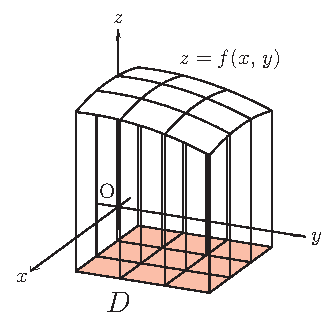
\includegraphics[width=6.5cm]{picture/juusekibun1.pdf} 
 \caption{マックのポテト}
\end{figure}

$D$を十分細かく分割すれば,
上に描いたマックのポテトのような立体の体積が$f(x, \, y)\:\mathrm{d}S$とみなすことができる.
これを領域$D$上すべての点で合計するのだから,
関数$z=f(x, \, y)$を領域$D$上で2重積分することで得られた値というのは
曲面$z=f(x, \, y)$と$D$の間の領域の体積を表していることになるというわけだ.
この場合でもこの値は負になることがある.
従って,この体積は符号付き体積とでも読んでおくべき量である.
ほとんど1変数関数のときと変わらないのである.

変数が増えても考えることは同じである.3変数関数$f(x, \, y, \, z)$をある領域$V$上で積分したければ,
まず$x, \, y, \, z$の微分$\mathrm{d}x, \, \mathrm{d}y, \, \mathrm{d}z$を考え,
これと$f(x, \, y, \, z)$との積$f(x, \, y, \, z)\:\mathrm{d}x\mathrm{d}y\mathrm{d}z$を作り,
そしてこれを$V$上全域にわたって足し合わせるのである.この値は
$$
\iiint_{V} f(x, \, y, \, z) \: \mathrm{d}x\mathrm{d}y\mathrm{d}z
$$
と書くことができるだろう.やはり,$\mathrm{d}x\mathrm{d}y\mathrm{d}z$という量が微小な体積を表しているのだと解釈できる.
したがってこれを$\mathrm{d}V$と置き換えてみると,この積分は
$$
\int_{V} f(x, \, y, \, z) \: \mathrm{d}V
$$
と書き換えられることになるというわけだ.
しかし,関数$f(x, \, y, \, z)$のグラフというのは4次元空間に存在するものであるから,
この積分を図に描けと言われてもそれは無理である.
しかし,計算することくらいは可能であろう.
変数が増えてくると,もはや積分を面積や体積などといった概念で解釈するのは不可能となる.
そのときはとりあえず1変数関数や2変数関数の積分と同じようなものを表しているのだろうと思っておくしかない.

\subsection{重積分の正確な定義}
さっき述べた定義は重積分の定義というよりは,その具体的なイメージである.
これでは定義としてあやふやなので,正確な定義を述べておこう.
変数の数がいくつでも同じやり方で定義するので,3重積分について述べておく.

$xyz$空間の領域$V$で定義された3変数関数$f(x, \, y, \, z)$について考える.
$V$はある範囲に収まった領域(つまり有界閉領域)としておき,
$V$を含むような十分大きな直方体$R$を考える.
\begin{align*}
R = \Set{ (x, \, y, \, z) | a_1\leq x \leq a_2 , \, b_1 \leq y \leq b_2 , \, c_1 \leq z \leq c_2 }
\end{align*}
とでも書いておこう.
そして,$R$上で定義された関数$f^* (x, \, y,\, z)$を
\begin{empheq}[left={f^*(x, \, y, \, z)=\empheqlbrace}]{alignat*=2}
f(x, \, y, \, z)  \quad & \Big( (x, \, y, \, z) \in V \Big) \\
0 \hspace{1cm} & \Big( (x, \, y, \, z) \not\in V \Big)
\end{empheq}
と定める.もともと$V$上でしか定義されていなかった関数の定義域を拡大したのだ.
$V$はどんな変な形をした領域かわかったものではない.
そこで,$V$の代わりに扱いやすい直方体を考えるのである.

さて,直方体$R$を分割しよう.そのような分割を$\varDelta$とおく.
\begin{empheq}[left={\varDelta : }]{align*}
a_1 & = x_0 < x_1 < \cdots < x_l = a_2 \\
b_1 & = y_0 < y_1 < \cdots < y_m = b_2 \\
c_1 & = z_0 < z_1 < \cdots < z_n = c_2 
\end{empheq}
というように表せるだろう.この分割により,$R$は微小直方体$R_{ijk}$に分割される.
\begin{align*}
R_{ijk} = \Set{ (x, \, y, \, z) | x_{i-1}\leq x \leq x_i , \, y_{j-1} \leq y \leq y_j , \, 
z_{k-1} \leq z \leq z_k }
\end{align*}
となる.さて,この微小直方体から1点$\mathrm{P} _{ijk} (p_i, \, p_j, \, p_k)$を任意にとり,
さらに$\varDelta x_i=x_i-x_{i-1} , \, \varDelta y_j = y_j - y_{j-1}, \, \varDelta z_k = z_k-z_{k-1}$
とおき,次のようなRiemann和\index[nidx]{Riemann@Riemann(リーマン)}
を考える.
\begin{align*}
\sum_{i, \, j, \, k} f^* (p_i, \, p_j, \, p_k) \varDelta x_i \varDelta y_j \varDelta z_k
\end{align*}
$\sum$の下に$i, \, j, \, k$と書いているのは,
$i, \, j, \, k$としてありうるものすべての和をとってくれという意味である.
いちいち$\sum$を3つも書かなくて済むのでこの書き方は便利である.
もし$\sum$を省略せずに書くのであれば,
\begin{align*}
\sum_{i=1}^{l} \sum_{j=1}^{m} \sum_{k=1}^{n} f^* (p_i, \, p_j, \, p_k) \varDelta x_i \varDelta y_j \varDelta z_k
\end{align*}
と表されるだろう.$i, \, j, \, k$はそれぞれ独立に動くので,どの$\sum$を先に計算しようと結果は変わらない.
そういうわけでさっきのような略記法が使えることになるのだ.

さて,このRiemann和に対して,各分割の幅を限りなく小さくしたときの極限を考えたい.
それには,$l, \, m, \, n \to \infty$と考えるか,あるいは
各微小直方体の体対角線(同じ面上にない頂点同士を結んだ線分)の長さの最大値$\delta$
が限りなく0に近づくと考えても同じことである.
すなわち,次のような極限を考えるのである.
\begin{align*}
\lim_{\delta \to 0} \sum_{i, \, j, \, k} f^* (p_i, \, p_j, \, p_k) \varDelta x_i \varDelta y_j \varDelta z_k
\end{align*}
もしこの極限が$\varDelta$や$\mathrm{P}_{ijk}$のとり方に依存せず,
一定の値に確定するのであれば,
$f(x, \, y, \, z)$は領域$V$上で\emph{可積分}\index[widx]{かせきぶん@可積分}であるといって,
その極限値を
\begin{align*}
\iiint_V f(x, \, y, \, z) \, \mathrm{d}x \mathrm{d} y \mathrm{d} z
\end{align*}
と表し,関数$f(x, \, y, \, z)$の領域$V$における\textbf{3重積分}と呼ぶ.

$x, \, y, \, z$というのは仮に用意した変数であって,別のものを用いてもよい.
そこで,後に学ぶ位置ベクトルを連想して,
$x, \, y, \, z$をまとめて$\bm{r}$という1つのベクトルで代表させて,積分を
\begin{align*}
\iiint_V f(x, \, y, \, z) \, \mathrm{d}^3 \bm{r}
\end{align*}
というように表すこともある.3乗のような記号がくっついているのは3重積分をイメージしてのことである.
あるいは,$\bm{r}$ではなく$\bm{x}$というベクトルで代表させれば
\begin{align*}
\iiint_V f(x, \, y, \, z) \, \mathrm{d}^3 \bm{x}
\end{align*}
というように表せる.上付きの3を省略してしまって
\begin{align*}
\iiint_V f(x, \, y, \, z) \, \mathrm{d} \bm{x}
\end{align*}
というように表すこともある.
書き方が違うだけで全部同じ積分を表す.混乱しないように気を付けよう.



ちょっと長くて混乱したかもしれないが,積分というのは結局
\begin{enumerate}
\item 積分領域を分割して
\item 分割された各領域から代表となる点をとり
\item その点における関数値とそこの領域の体積をかけて
\item その量を領域全体にわたって足し合わせて(ここまででRiemann和)\index[nidx]{Riemann@Riemann(リーマン)}
\item 各分割幅を限りなく小さくするような極限を考える
\end{enumerate}
だけなのである.
変数が増えようが,積分領域が変わろうが,
積分する対象が変わろうが,これだけは変わらない.
\footnote{ただし,この考えがよくないとして,あらためて積分の理論を組み立てなおした積分もあって,
それはLebesgue\index[nidx]{Lebesgue@Lebesgue(ルベーグ)}
積分と呼ばれている.この場合はもちろんこの考え方は当てはまらない.}
\begin{itembox}[l]{検討}
さっきやった方法では,$R$のうち,$V$の外側では値が0になるような関数$f^*(x, \, y, \, z)$を考えた.
これは,直方体$R$の$V$の外側の部分で積分値に変化がないようにするためである.

さて,``連続関数は可積分である''というのは有名な事実であるが,
元の関数$f(x, \, y, \, z)$が連続関数であっても,$f^*(x, \, y, \, z)$は$V$の境界線のところで
不連続になってしまうことがある.
このことは,可積分性に影響を与えることはあるだろうか?
\end{itembox}

\subsection{重積分の計算方法}
重積分の具体的なイメージは湧いただろうか? しかし,
イメージができたところで重積分が実際に計算できるかと言われたら話は別である.

ここでは領域$D$を
\begin{align*}
D= \Set{ (x, \, y) | 0 \leq x \leq y , \, 0 \leq y \leq 1}
\end{align*}
として,$D$上で関数$z = x + y$を積分してみる.
\begin{align*}
\iint_{D} z \, \mathrm{d}x \mathrm{d}y & = \iint_{D} (x+y) \, \mathrm{d}x \mathrm{d}y \\
& = \int_0^1 \left( \int_0^y (x+y) \, \mathrm{d}x \right) \mathrm{d}y \\
& = \int_0^1 \left[ \frac{1}{2} x^2 + xy \right]_0^y \mathrm{d}y \\
& = \int_0^1 \frac{3}{2} y^2 \, \mathrm{d}y \\
& = \left[ \frac{1}{2} y^3 \right]_0^1 = \frac{1}{2}
\end{align*}
普通に計算したように見えて,実はとても巧妙な技巧を使ってやっている.
いわゆる\emph{累次積分}\index[widx]{るいじせきぶん@累次積分}と呼ばれる手法である.
累次積分の真価は1行目から3行目あたりのところの式変形である.
あたかも$x$と$y$がまったく無関係に独立に変化しているかのように扱われているではないか!

実は,このような式変形ができるためには条件があって,
それは,積分領域を表す変数の変域のうちどれかが他の変数を含まない閉区間でなければならないというものである.
さっきの例では$x$の範囲は$0 \leq x \leq y$と,$y$を含んでいた.しかし,$y$の変域は$0 \leq y \leq 1$と,
$x$をまったく含んでいない.累次積分はこういう場合に使える技法である.
ただ単純に1変数関数での積分を2回やるだけである.
とはいえ,この非常に便利な技法が使えることをきちんと証明しようとすると,
やっぱり$\varepsilon - \delta$論法が必要になってくる.

きちんとまとめておくと,関数$f(x, \, y)$と領域$D$について,もし積分領域$D$が
\begin{align*}
D = \Set{ (x, \, y) | a \leq x \leq b , \, g(x) \leq y \leq h(x) }
\end{align*}
という形式で書けたとするならば,
\begin{align}
\iint_D f(x, \, y) \, \mathrm{d} x \mathrm{d} y
= \int_a^b \left( \int_{g(x)}^{h(x)} f(x, \, y) \, \mathrm{d} y \right) \mathrm{d}x 
\label{eq:ruijisekibuny}
\end{align}
と計算できる.この場合,$y$で積分するときには$x$はさも定数であるかのようにみなす.
偏微分のときと同じようなイメージである.
$x$で積分するときには$y$はすでに式中からなくなっており,
ただの定積分として計算できる.
なお,式(\ref{eq:ruijisekibuny})の右辺の積分を
\begin{align*}
\int_a^b \mathrm{d}x  \int_{g(x)}^{h(x)} f(x, \, y) \, \mathrm{d} y 
\end{align*}
と書き表すことがある.書き方が違ってもそれは式(\ref{eq:ruijisekibuny})
同じ積分を表している.単に書き方の問題である.

同じように領域$D$が
\begin{align*}
D = \Set{ (x, \, y) | g(y) \leq x \leq h(y) , \, a \leq y \leq b }
\end{align*}
という形式で書けたとするならば,
\begin{align}
\iint_D f(x, \, y) \, \mathrm{d} x \mathrm{d} y
= \int_a^b \left( \int_{g(y)}^{h(y)} f(x, \, y) \, \mathrm{d} x \right) \mathrm{d}y
\label{eq:ruijisekibunx}
\end{align}
と計算できることになる.
例によって,この式の右辺の積分は
\begin{align*}
\int_a^b \mathrm{d}y  \int_{g(y)}^{h(y)} f(x, \, y) \, \mathrm{d} x 
\end{align*}
と書かれることがある.
\begin{itembox}[l]{課題}
$xy$平面上での領域$D$を
\begin{align*}
D= \Set{ (x, \, y) | 0\leq y\leq 1-x , \, 0 \leq x \leq 1 }
\end{align*}
として,2重積分
\begin{align*}
\iint_{D} (x^2+y^2) \: \mathrm{d}x \mathrm{d}y
\end{align*}
を求めよ.

また,$xy$平面上の領域$D$を
\begin{align*}
D = \Set{ (x, \, y) | 0 \leq y \leq 1 , \, y \leq x \leq 1 }
\end{align*}
としたとき,2重積分
\begin{align*}
\iint_D \exp \left( \frac{y}{x} \right) \, \mathrm{d}x \mathrm{d}y
\end{align*}
を求めよ.(ヒント:$D$を図示してみよ)
\end{itembox}

\subsection{重積分の変数変換}
1変数関数の積分において,計算を進めるための技法として,置換積分法というのがあった.

$x$の関数$f(x)$があり,変数$x$が別の変数$t$の関数であり,$x=g(t)$と表せたとする.
$x$の微分$\mathrm{d}x$が
\begin{align*}
\mathrm{d}x = \frac{ \mathrm{d} x}{\mathrm{d} t } \mathrm{d} t 
\end{align*}
と表せることを利用して,$g(\alpha) = a, \, g(\beta) = b$となったとするとき
\begin{align}
\int_a^b f(x) \, \mathrm{d} x = \int_{\alpha}^{\beta} f(g(t))
\frac{ \mathrm{d} x}{\mathrm{d} t } \mathrm{d} t 
\label{eq:tikansekibun}
\end{align}
と計算するのであった.
この技法を重積分にも取り入れたい.
しかし,これは簡単そうで意外と面倒な事柄がたくさんあるのである.
なお,ここからの内容は先に第\ref{vecterop}章を読んでから取り組むことを推奨する.

\subsubsection{ヤコビ行列の登場}
話を簡単にするため,ここからは2重積分について考える.

$x, \, y$の2変数関数$f(x, \, y)$があり,変数$x, \, y$は別の変数$u, \, v$によって
$x=\varphi (u, \, v), \, y=\psi (u, \, v)$と表されていたとする.
ただし,各$(u, \, v)$と$(x, \, y)$が1対1に対応しているとしよう.
$x, \, y$の全微分はそれぞれ
\begin{align*}
\mathrm{d} x = \frac{\partial x}{\partial u} \mathrm{d}u + \frac{\partial x}{\partial v} \mathrm{d}v \\
\mathrm{d} y = \frac{\partial y}{\partial u} \mathrm{d}u + \frac{\partial y}{\partial v} \mathrm{d}v
\end{align*}
となるのだったから,
\begin{align*}
\mathrm{d}x \mathrm{d}y & = \left( 
\frac{\partial x}{\partial u} \mathrm{d}u + \frac{\partial x}{\partial v} \mathrm{d}v \right) 
\left( \frac{\partial y}{\partial u} \mathrm{d}u + \frac{\partial y}{\partial v} \mathrm{d}v \right) \\
& = \frac{\partial x}{\partial u} \frac{\partial y}{\partial u} (\mathrm{d}u)^2
+ \left( \frac{\partial x}{\partial u}\frac{\partial y}{\partial v} + 
\frac{\partial x}{\partial v}\frac{\partial y}{\partial u} \right) \mathrm{d}u \mathrm{d}v +
\frac{\partial x}{\partial v}\frac{\partial y}{\partial v} (\mathrm{d}v)^2
\end{align*}
と計算できそうだが,残念ながらこれは間違いである.
というのも,左辺は$x, \, y$を基準とした座標系,すなわち直交直線座標系で測ったときの
微小面積である.これを$u, \, v$を基準とした座標系
で測ったときには単純に積をとればいいというわけにはいかないのだ.
詳しいことは述べないので自分で考えてもらいたい.

ではどうすればいいかというと,全微分の式を行列形式で書き表してやって,
\begin{align}
\left[
\begin{array}{c}
\mathrm{d} x \\
\mathrm{d} y
\end{array}
\right]
= \left[
\renewcommand{\arraystretch}{2}
\begin{array}{cc}
\dfrac{ \partial x}{\partial u} & \dfrac{ \partial x}{\partial v} \\
\dfrac{ \partial y}{\partial u} & \dfrac{ \partial y}{\partial v} \\
\end{array}
\renewcommand{\arraystretch}{1}
\right]
\left[
\begin{array}{c}
\mathrm{d}u \\
\mathrm{d} v
\end{array}
\right]
\label{eq:jacobima}
\end{align}
としてみる.式(\ref{eq:jacobima})中に出てきた行列
\begin{align}
J = \left[
\renewcommand{\arraystretch}{2}
\begin{array}{cc}
\dfrac{ \partial x}{\partial u} & \dfrac{ \partial x}{\partial v} \\
\dfrac{ \partial y}{\partial u} & \dfrac{ \partial y}{\partial v} \\
\end{array}
\renewcommand{\arraystretch}{1}
\right]
\label{eq:jacobimatrix}
\end{align}
を座標変換$(u, \, v) \mapsto (x, \, y)$
\footnote{記号「$\mapsto$」は変換によって
$(u, \, v)$が$(x, \, y)$に対応することを指し示すために使われる記号である.}
の\emph{ヤコビ行列}\index[widx]{やこびあん@ヤコビ行列}と呼び,
その行列式
\begin{align}
\det J = \det \left[
\renewcommand{\arraystretch}{2}
\begin{array}{cc}
\dfrac{ \partial x}{\partial u} & \dfrac{ \partial x}{\partial v} \\
\dfrac{ \partial y}{\partial u} & \dfrac{ \partial y}{\partial v} \\
\end{array}
\renewcommand{\arraystretch}{1}
\right] = \left \lvert
\renewcommand{\arraystretch}{2}
\begin{array}{cc}
\dfrac{ \partial x}{\partial u} & \dfrac{ \partial x}{\partial v} \\
\dfrac{ \partial y}{\partial u} & \dfrac{ \partial y}{\partial v} \\
\end{array}
\renewcommand{\arraystretch}{1}
\right \rvert
\label{eq:jacobian}
\end{align}
を座標変換$(u, \, v) \mapsto (x, \, y)$の
\emph{ヤコビ行列式},\index[widx]{やこびぎょうれつしき@ヤコビ行列式|see{ヤコビアン}}
もしくは\emph{ヤコビアン}\index[widx]{やこびあん@ヤコビアン}と呼ぶ.
\footnote{名前のついた行列の行列式を表すとき,よく語尾を-ianと書き換えることが多い.
Jacobi\index[nidx]{Jacobi@Jacobi(ヤコビ)}行列の行列式ならJacobianという具合である.}

よく使うのはヤコビ行列よりもヤコビアンの方であり,ヤコビ行列が議論に出てくることはあまりない.
そういう事情からか,ヤコビ行列とヤコビアンがごっちゃになっていることがある.
文脈によってどちらを指しているのかきちんと見分ける癖をつけておこう.

また,ヤコビアンは次のような形で表されることもある.
\begin{align}
\frac{ \partial (x, \, y)}{ \partial (u, \, v) } = 
\left \lvert
\renewcommand{\arraystretch}{2}
\begin{array}{cc}
\dfrac{ \partial x}{\partial u} & \dfrac{ \partial x}{\partial v} \\
\dfrac{ \partial y}{\partial u} & \dfrac{ \partial y}{\partial v} \\
\end{array}
\renewcommand{\arraystretch}{1}
\right \rvert
\label{eq:jacobian2}
\end{align}
ヤコビアンは偏導関数を書き並べた行列の行列式であるから,
これを偏微分の拡張であるかのようにみなすイメージである.

さて,重積分の変数変換の文脈では,座標変換に対応したヤコビアンに対し,
\begin{align}
\mathrm{d} x \mathrm{d}y = \lvert \det J \rvert \, \mathrm{d} u \mathrm{d}v
\label{eq:jacobimenseki}
\end{align}
としてやるのが正しい.右辺の$\lvert \; \cdot \; \rvert$は絶対値を表す記号である.
行列式を表す記号と混同しないようにしてほしい.
なぜこれでうまくいくのだろう?

2つのベクトル
\begin{align*}
\left[
\renewcommand{\arraystretch}{2}
\begin{array}{c}
\dfrac{ \partial x}{\partial u} \\
\dfrac{ \partial y}{\partial u}
\end{array}
\right]
, \; \left[
\renewcommand{\arraystretch}{2}
\begin{array}{c}
\dfrac{ \partial x}{\partial v} \\
\dfrac{ \partial y}{\partial v}
\end{array}
\right]
\renewcommand{\arraystretch}{1}
\end{align*}
を見てみると,これは変数$u, \, v$が微小変化したときの$x, \, y$の変化の方向を表すベクトルである.
ヤコビ行列$J$を構成するベクトルは,変換後の座標系において$u , \, v$が微小変化したとき,
それが変換前の座標系ではどういう方向に変化するかを表していることになる.
線形代数学の知識によれば,ヤコビアン$\det J$はそれらのベクトルが張る平行四辺形の面積を表していることになる.
この``面積''というのはいわゆる符号付き面積のことだから,
絶対値を付けて正の値になるように調整していることになる.
1変数関数の置換積分のときには絶対値などは付けなかった.
これは,被積分関数が1変数関数であったため,変数の変化に向きがあったのだが,
重積分においては複数の変数が自由気ままに動き回り,変数の変化に向きなどないからである.

まとめよう.2変数関数$f(x, \, y)$を領域$D$上で積分するとき,
もし$x, \, y$が$x=\varphi (u, \, v) , \, y = \psi (u, \, v)$と表されていて,
かつ各$(u, \, v)$に対して$(x, \, y)$が1対1に対応しているとする.
点$(x, \, y)$が$D$上を動くときの点$(u, \, v)$が動く範囲を$D'$とすれば,
$D$上の各点$(x, \, y)$と$D'$上の点$(u, \, v)$が完全に1対1に対応することになる.
このとき,座標変換$(u, \, v) \mapsto (x, \, y)$のヤコビ行列を$J$として
\begin{align}
\iint_D f(x, \, y) \, \mathrm{d}x \mathrm{d} y 
= \iint_{D'} f( \varphi (u, \, v) , \, \psi (u, \, v) ) \, \lvert \det J \rvert \, \mathrm{d}u \mathrm{d}v
\label{eq:jusekibunhenkan}
\end{align}
という計算をしてやればよいということである.
式(\ref{eq:jacobian2})の表現方法を採用してみると
\begin{align}
\iint_D f(x, \, y) \, \mathrm{d}x \mathrm{d} y 
= \iint_{D'} f( \varphi (u, \, v) , \, \psi (u, \, v) ) 
\left \lvert \frac{ \partial (x, \, y) } { \partial (u, \, v) } \right \rvert \mathrm{d}u \mathrm{d}v
\label{eq:jusekibunhenkan2}
\end{align}
と表されることになる.こうしてみると,ヤコビアンを用いた重積分の変数変換が
1変数関数における置換積分法の拡張になっていることが一目瞭然である.

変数変換によって積分の式が余計にややこしくなったように見えるが,
右辺の方が簡単になるようにうまく座標変換を定義してやるのが腕の見せ所である.

今回は2重積分で話をしたが,変数の数が増えてもやることは同じである.
ただヤコビ行列の次数が増えていくだけである.

\subsubsection{具体例}
一般的な議論が済んだところで,ヤコビアンの力を実感するためにいくつか問題を解いてみよう.

$xy$平面上の領域$D$を
\begin{align*}
D = \Set{ (x, \, y) | 1 \leq  x+y \leq 2 , \, 1 \leq x-y \leq 3 }
\end{align*}
と定めたとき,関数$z=x^2-y^2$の$D$上での2重積分
を求めてみよう.
\begin{align*}
u = x + y \\
v = x - y 
\end{align*}
とおき,座標変換$(u, \, v) \mapsto (x, \, y)$を考える.
\begin{align*}
x = \frac{1}{2} u + \frac{1}{2} v \\
y = \frac{1}{2} u - \frac{1}{2} v
\end{align*}
と書けるので,
この座標変換のヤコビ行列$J$は
\begin{align*}
J = \left[
\renewcommand{\arraystretch}{2}
\begin{array}{cc}
\dfrac{ \partial x}{\partial u} & \dfrac{ \partial x}{\partial v} \\
\dfrac{ \partial y}{\partial u} & \dfrac{ \partial y}{\partial v} \\
\end{array}
\renewcommand{\arraystretch}{1}
\right] = \left[
\renewcommand{\arraystretch}{2}
\begin{array}{cc}
\dfrac{1}{2} & \dfrac{1}{2} \\
\dfrac{1}{2} & - \dfrac{1}{2}
\end{array}
\renewcommand{\arraystretch}{1}
\right]
\end{align*}
となり,この座標変換のヤコビアンは
\begin{align*}
\frac{ \partial ( x , \, y ) }{\partial (u, \, v ) } 
= \left \lvert
\renewcommand{\arraystretch}{2}
\begin{array}{cc}
\dfrac{1}{2} & \dfrac{1}{2} \\
\dfrac{1}{2} & - \dfrac{1}{2}
\end{array}
\renewcommand{\arraystretch}{1}
\right \rvert
= - \frac{1}{2}
\end{align*}
と計算できる.
\begin{align*}
D' = \Set{ (u , \, v) | 1 \leq u \leq 2 , \, 1 \leq v \leq 3 }
\end{align*}
とおけば,$D$上の各点$(x, \, y)$と$D'$上の各点$(u, \, v)$は1対1に対応し,
$z=x^2-y^2=(x+y)(x-y)=uv$と書けるので
\begin{align*}
\iint_D z \, \mathrm{d}x\mathrm{d}y 
& = \iint_{D'} uv \left \lvert - \frac{1}{2} \right \rvert \mathrm{d}u\mathrm{d}v \\
& = \int_1^3 \mathrm{d}v \int_1^2 \frac{1}{2} uv \, \mathrm{d} u \\
& = \int_1^3 \mathrm{d}v \left[ \frac{1}{4} u^2 v \right]_1^2 \\
& = \int_1^3 \frac{3}{4} v \, \mathrm{d}v \\
& = \left[ \frac{3}{8} v^2 \right]_1^3 \\
& = 3
\end{align*}
と計算できることになる.
このくらいの積分なら変数変換を使わずとも求めるのはさほど難易度は高くないのだが,
計算が煩雑になり,とても面倒である.

次に,$xyz$空間の領域$V$を
\begin{align*}
V = \Set{ (x, \, y, \, z ) | x^2 + y^2 + z^2 \leq R^2 }
\end{align*}
としたとき,関数$u=1$の$V$上での3重積分
を求めてみよう.
ただし$R$は正の定数とする.

点$(x, \, y, \, z)$を極座標系$(r, \, \theta, \, \varphi)$で表し,
\begin{align*}
x & = r \sin \theta \cos \varphi \\
y & = r \sin \theta \sin \varphi \\
z & = r \cos \theta 
\end{align*}
とおく.
この座標変換$(r, \, \theta , \, \varphi ) \mapsto (x, \, y, \, z)$のヤコビ行列$J$は
\begin{align*}
J = \left[ 
\renewcommand{\arraystretch}{2}
\begin{array}{ccc} 
\dfrac{ \partial x}{\partial r} & \dfrac{ \partial x}{\partial \theta} 
& \dfrac{ \partial x}{\partial \varphi} \\
\dfrac{ \partial y}{\partial r} & \dfrac{ \partial y}{\partial \theta} 
& \dfrac{ \partial y}{\partial \varphi} \\
\dfrac{ \partial z}{\partial r} & \dfrac{ \partial z}{\partial \theta} 
& \dfrac{ \partial z}{\partial \varphi} 
\end{array}
\renewcommand{\arraystretch}{1}
\right] = \left[
\begin{array}{ccc}
\sin \theta \cos \varphi & r \cos \theta \cos \varphi & - r \sin \theta \sin \varphi \\
\sin \theta \sin \varphi & r \cos \theta \sin \varphi & r \sin \theta \cos \varphi \\
\cos \theta & -r \sin \theta & 0
\end{array}
\right]
\end{align*}
となる.
よって,座標変換$(r, \, \theta , \, \varphi ) \mapsto (x, \, y, \, z)$のヤコビアンは,
余因子展開等を駆使して頑張って計算すると
\begin{align*}
\frac{ \partial (x, \, y, \, z) } { \partial (r, \, \theta , \, \varphi ) }
& = \left \lvert
\begin{array}{ccc}
\sin \theta \cos \varphi & r \cos \theta \cos \varphi & - r \sin \theta \sin \varphi \\
\sin \theta \sin \varphi & r \cos \theta \sin \varphi & r \sin \theta \cos \varphi \\
\cos \theta & -r \sin \theta & 0
\end{array}
\right \rvert \\
& = (-1)^{3+1} \cos \theta 
\left \lvert 
\begin{array}{cc}
r \cos \theta \cos \varphi & - r \sin \theta \sin \varphi \\
r \cos \theta \sin \varphi & r \sin \theta \cos \varphi 
\end{array}
\right \rvert \\
& \hspace{1cm} + (-1)^{3+2} ( - r \sin \theta ) 
\left \lvert 
\begin{array}{cc} 
\sin \theta \cos \varphi & - r \sin \theta \sin \varphi \\
\sin \theta \sin \varphi & r \sin \theta \cos \varphi 
\end{array}
\right \rvert \\
& = r^2 \cos \theta ( \sin \theta \cos \theta \cos ^2 \varphi 
+ \sin \theta \cos \theta \sin^2 \varphi ) \\ 
& \hspace{2cm} + r^2 \sin^3 \theta ( \cos ^2 \varphi + \sin ^2 \varphi ) \\
& = r^2 \sin \theta \cos ^2 \theta + r^2 \sin ^3 \theta \\
& = r^2 \sin \theta  
\end{align*}
となる.計算過程は面倒だが,結果はきれいな式となった.一生に一度は手を動かして計算しておこう.
その後は結果を暗記しておけばよい.

さて,
\begin{align*}
E = \Set{ (r, \, \theta , \, \varphi) 
| 0 \leq r \leq R , \, 0 \leq \theta \leq \pi , \, 0 \leq \varphi \leq 2 \pi }
\end{align*}
とおけば,$V$上の点$(x, \, y, \, z)$と$E$上の点$(r, \, \theta , \, \varphi)$
は1対1には対応しない.
しかし,1対1対応が崩れるような点は``ごくわずか''であり,
実はこのような場合でも変数変換は問題なく行えることが知られている.
このあたりの繊細な議論は本書の求めるものではないので考えないことにして,
さっさと積分を求めてしまおう.
\begin{align*}
\iiint_V 1 \, \mathrm{d} x \mathrm{d} y \mathrm{d} z 
& = \iiint_E \lvert r^2 \sin \theta \rvert 
\, \mathrm{d} r \mathrm{d} \theta \mathrm{d} \varphi \\
& = \int_0^{2\pi} \mathrm{d} \varphi \int_0^{\pi} \mathrm{d} \theta
\int_0^R r^2 \sin \theta \, \mathrm{d}r \\
& = \int_0^{2\pi} \mathrm{d} \varphi \int_0^{\pi} \mathrm{d} \theta
\left[ \frac{1}{3} r^3 \sin \theta \right]_0^R \\
& = \int_0^{2\pi} \mathrm{d} \varphi 
\int_0^{\pi} \frac{R^3}{3} \sin \theta \, \mathrm{d} \theta \\
& = \int_0^{2\pi} \mathrm{d} \varphi 
\left[ - \frac{R^3}{3} \cos \theta \right]_0^{\pi} \\
& = \int_0^{2\pi} \frac{2}{3} R^3 \, \mathrm{d} \varphi \\
& = \left[ \frac{2}{3} R^3 \varphi \right]_0^{2\pi} \\
& = \frac{4}{3} \pi R^3
\end{align*}
と,長らく慣れ親しんできた球の体積の公式が求められたことになる.

3次元の極座標変換におけるヤコビアンは$r^2 \sin \theta$であった.
2次元の極座標変換
\begin{align*}
x = r \cos \theta \\
y = r \sin \theta
\end{align*}
においてはヤコビアンは$r$となる.
計算は簡単なのでぜひともやっておき,結果を頭に叩き込んでおいてほしい.

\section{\textrm{Dirac}の$\delta$関数}
物理では,モノの位置を点で表現することがある.
質点や点電荷などがいい例である.
これらの概念は非常に便利である反面,
その密度を扱うときにちょっと困ったことが起こる.

とりあえず点電荷で考えてみよう.話を簡単にするために,1次元で考えてみる.
位置$a$に電荷量$q$の点電荷があるとする.
この点電荷の電荷密度を$\rho(x)$とおくと,
\begin{align}
q = \int_{- \infty}^{\infty} \rho ( x ) \, \mathrm{d} x 
\label{eq:denkamitudo}
\end{align}
が成り立っているはずである.
今回は積分範囲を$x$軸全体にしたが,点$a$さえ含まれていればどんな積分区間でも構わない.

ここからが問題である.
電荷は位置$a$にしか存在しないのだから,そこ以外の電荷密度はすべて0になっているはずで,
\begin{align*}
\rho ( x) = 0 \quad (\text{ただし$x \neq a$})
\end{align*}
が成り立つ.では$\rho (a)$はいくつだろう? $\rho (a) = q$とでもしておけばよさそうな気がする.
しかしこれでは式(\ref{eq:denkamitudo})を成り立たせることはできない.
それどころか$\rho(a)$をどんな値に定めようが無駄である.
いくら積分区間に点$a$が含まれていようとも,
区間を分割したときの幅が微小であるために1点だけで正で有限の値を持ったとしても
それが積分値に影響を与えないからだ.
つまり,式(\ref{eq:denkamitudo})をみたし,
かつ点$a$以外ではその値が0になるような関数は存在しないことになる.
これは困る.点電荷や質点は非常によく使う概念であるのにその密度がわからないというのだ!

\subsection{\textrm{Dirac}の解決策}
上記のような問題を解決するために,
物理学者Dirac\index[nidx]{Dirac@Dirac(ディラック)}
は次のような性質をみたす``関数''$\delta (x)$を編み出した.
\footnote{これは$\delta$関数の正確な出自とは違う.
Dirac自身は量子力学での問題を解決するのに$\delta$関数を利用した.}
\begin{itembox}[l]{定義}
任意の連続関数$f(x)$に対して
\begin{align}
\int_{-\infty}^{\infty} f(x) \, \delta (x) \, \mathrm{d}x = f(0)
\label{eq:deltadisdef}
\end{align}
をみたす``関数''$\delta(x)$を\textbf{Diracの$\delta$関数},
\index[widx]{でるたかんすう@$\delta$関数}
もしくは単に\textbf{$\delta$関数}と呼ぶ.
\end{itembox}
この``関数''を使えば,点$a$に存在する点電荷$q$の電荷密度は
\begin{align}
\rho (x) = q \, \delta ( x-a )
\label{eq:denkamitudodelta}
\end{align}
と求めることができる.
この$\rho(x)$が式(\ref{eq:denkamitudo})をみたすことは
置換積分法によって簡単に示すことができる.

また,$\delta$関数は次のような性質を持っている.
\begin{align}
\delta ( x) = \left \{
\begin{aligned} 
0 \hspace{4.2mm} & (x \neq 0) \\
\infty \quad & (x = 0)
\end{aligned}
\right.
\label{eq:deltainfty}
\end{align}
$\delta(0)$の値が有限の値では目的の性質が得られなかったので,
とりあえず$\infty$ということにしてある.この時点で怪しい香りがしてくる.
こんなものは性質とは言わない.$\delta$関数は積分して初めて意味を持つ.
こんな``関数''を関数として認めてしまっていいだろうか? ``編み出した''というのがどうもうさんくさい.
ずっと``関数''と表記していたのはこのためである.
ないものをあるとかたくなに言い張っているだけにしか見えない.
そんなうさんくさい概念を議論に持ち込んでいいものだろうか? この問題は多くの数学者,
物理学者を悩ませた.
$\delta$関数は物理学の役に立つし,必要不可欠なものである.
しかしその実態は何なのか? どう定義したらいいのか? ところが,それが解決されるのは案外早く,
わずか10年あまり後のことであった.
$\delta$関数などというわけのわからない概念を
関数の概念を拡張することによって定式化してみせたのである.
そのように拡張された関数のことを\emph{超関数}と呼ぶ.
通常の関数は英語ではfunctionというが,
超関数は英語ではdistributionということが多い.
しかし,超関数の定式化のやり方はいろいろあって,
その手法によっては違った呼ばれ方をされることもある.
超関数の詳しい定義は本書では取り上げることはしないが,
とりあえず$\delta$関数は数学的に定式化されたものであり,
決してよくわからない怪しい概念ではないということを理解しておいてほしい.
初学者向けに$\delta$関数のわけのわからなさを強調して話されることがよくあるが,
それはあくまで$\delta$関数が通常の意味での関数ではないということを伝えたいだけなのである.

\subsection{$\delta$関数の初等関数による近似}
いくら$\delta$関数が数学的に定式化されているとはいっても,
つかみどころのない不思議な関数であることには違いない.
そういうわけで,$\delta$関数をよく知っている関数の極限として考えるという方法がある.
たくさんあるが,その中でもよく見るものをピックアップしておこう.
\begin{align}
\phi_n (x) & = \left \{
\begin{aligned}
& \, n \quad & \left( \lvert x \rvert \leq \frac{1}{2n} \right) \\
& \, 0 \quad & \left( \lvert x \rvert > \frac{1}{2n} \right) 
\end{aligned}
\right. \\
\phi_n(x) & = \frac{ \sin nx}{\pi x} \\
\phi_n(x) & = \sqrt{ \frac{ n}{\pi}} \exp ( - nx^2)
\end{align}
これらの関数の$n \to \infty$としたときの極限として$\delta$関数を考えるのである.
これらの関数は$- \infty < x < \infty$の範囲で積分したときに常にその値が1になっているし,
\footnote{さらっと言っているがこれを厳密に証明するのは案外難しかったりする.}
なおかつ$x \neq 0$の範囲では$n \to \infty$としたときにその関数値が0に収束し,
$x = 0$のところでは$\infty$に発散する.
まさに$\delta$関数と同じような性質を持っているのである.
$n$をかなり大きめの有限の値にしておいて,$\delta$関数の代わりに
これらの関数を用いれば,完璧にではないにせよ
$\delta$関数のような関数を扱えることになる.
よく知っている初等関数の範囲で扱えるのが利点である.

\subsection{$\delta$関数の\textrm{Fourier}積分表示}
$\delta$関数のちょっと特殊な表現として,
次のようなものがある.
\begin{align}
\delta ( x ) = \frac{1}{2\pi} \int_{-\infty}^{\infty} \exp ( ikx) \, \mathrm{d}k
\label{eq:deltafourier}
\end{align}
なぜこの表現が特別視されているかというと,
この形が本書でカットしたFourier\index[nidx]{Fourier@Fourier(フーリエ)}
変換に深く結びついているからである.

なお,積分区間を有限にしたものであれば積分を実際に求めることができて,
\begin{align*}
\frac{1}{2\pi} \int_{-n}^{n} \exp ( ikx) \, \mathrm{d}k 
& = \frac{1}{2 \pi} \left[ \frac{1}{ix} \exp ( ikx) \right]_{-n}^n \\
& = \frac{1}{2 \pi ix} ( \exp ( inx ) - \exp( - inx) ) \\
& = \frac{ \sin nx} { \pi x}
\end{align*}
となる.Eulerの公式を思い出してほしい.
この式は先ほど説明した近似表現の1つである.
この式で$n \to \infty$としてやれば$\delta$関数が得られるのであった.
しかし,ここで重要なのは積分の形で書かれていることである.
Fourier変換を学んでみればそのあたりははっきりとわかるだろう.
そういうわけで,式(\ref{eq:deltafourier})は$\delta$関数の
\textbf{Fourier積分表示}と呼ばれている. 
\index[widx]{でるたかんすう@$\delta$関数!のふーりえせきぶんひょうじ@---のFourier積分表示}

\subsection{3次元での$\delta$関数}
先ほどやったのは1次元での$\delta$関数である.
しかし実際に点電荷の電荷密度などで利用するためには3次元でなくてはならない.
それはそんなに難しい話ではない.

点$( a, \, b, \, c)$に点電荷$q$が存在していることを表すには,
その電荷密度$\rho( x, \, y, \, z)$を$\delta$関数を使って次のように
表してやればいい.
\begin{align}
\rho ( x, \, y, \, z ) = q \, \delta( x -a ) \, \delta ( y-b) \, \delta( z-c)
\label{eq:deltamitudo3d}
\end{align}
このようにしてやれば,領域$V$が点$( a, \, b, \, c)$を含むとき
\begin{align}
\int_V \rho(x, \, y, \, z) \, \mathrm{d} V = q
\label{eq:delta3d}
\end{align}
は問題なく成り立つし,点$(a, \, b, \, c)$以外のところでは$\rho( x, \, y, \, z)=0$
が常に成り立っている.しかし,$x=a$で$y \neq b$などといった場合に少し困るが,
この際そういう細かいことは気にしないことにする.

また,いちいち$\delta$関数を3つも書くのは面倒なので,
\begin{align*}
 \delta ( \bm{r} ) , \, \delta ^{(3)} ( \bm{r})
 \end{align*}
 などと略記されることがある.書きたいことの意味はわかるだろう.
 この記法に従えば,位置$\bm{a}$にある点電荷$q$の電荷密度$\rho(\bm{r})$は
 \begin{align}
 \rho(\bm{r} ) = q \, \delta( \bm{r} - \bm{a} ) = q \, \delta^{(3) } ( \bm{r} - \bm{a})
 \label{eq:ryakkidelta}
 \end{align}
 と表せる.やっぱり表記は簡便な方がいい.
 
 $\delta$関数はもっとたくさんの面白い性質を秘めているのだが,
 そのあたりは類書に譲ることにしよう.
 物理学を学んでいればいずれまた遭遇するだろう.